% !TEX root = pfe-book4.tex
%!TEX TS-program = pdflatex
%!TEX encoding = UTF-8 Unicode


\cleardoublepage
%\mainmatter
\chapter{Soft Electromagnetic Radiation}
\label{ch-01}

\section{Exchange of Energy by Radiation}
\emph{Soft electromagnetic radiation} is that with wavelengths lying roughly in the interval from 0.1 to 100 micrometres. Also, bear in mind that when we speak of soft radiation we mean electromagnetic waves not dealt with in radio engineering. This stipulation is important because purely radio-engineering methods permit one to dip into the region of soft radiation. The soft radiation also rather frequently goes by the simple term ``light''. When applying that term, one must bear in mind that visible light occupies only a very narrow section of wavelengths -- for the ``average'' human eye it lies between 380 and 780 nanometres (or from 0.38 to 0.78 micrometres).

In future, whenever we have the occasion to speak of ``light'', we will do so in the broad sense of the word because the laws that hold true for the visible portion of the spectrum remain true for all other representatives of soft radiation.

Also note that radiation with shorter wavelengths than visible light is called \emph{ultraviolet radiation}; the longer wavelengths are termed \emph{infrared radiation}.

We can now turn to the topic of our discussion. It will be recalled that there are three modes of heat transfer. They are called heat conduction, thermal convection,
and thermal radiation. In order to study the exchange of energy that occurs in thermal radiation, we will have to  examine the behaviour of bodies in a vacuum (where convection is impossible) separated by a certain distance (this is to exclude the conduction of heat).

Experiments have shown that if two or more bodies form a closed system (the reader will recall that this means the absence of any exchange of energy between objects not in the system), the temperatures of the bodies equal out. Each one of the bodies of the system is at the same time a radiator and an absorber. What occur are numberless transitions of atoms and molecules from a higher level to a lower level (such events involve the emission of photons) and from a lower level to a higher level (photons are absorbed). Photons of all energies (or, what is the same thing, electromagnetic waves of all wavelengths) participate in these exchanges.

Quite naturally, the body does not absorb all the energy falling on it. There may be bodies that scatter more energy or transmit certain wavelengths. But this is of no consequence because sooner or later a thermal equilibrium is established nevertheless.

The condition of thermal equilibrium requires that the ratio of the energy of absorption to the energy of emission be the same for all wavelengths. This theorem was rigorously demonstrated in 1860 by the German physicist Gustav Robert Kirchhoff (1824-1887). The ratio can change for different temperatures, but if the temperature is fixed, then it is the same for photons of all energies.

This is a clear enough theorem and hardly needs any demonstration of proof. The idea behind the law is that the number of absorbed photons of a given kind (that is, of a definite energy) is equal, in the case of thermal equilibrium, to the number of radiated photons of that particular kind. From this we get the following rule: if an object is a strong absorber of any kind of rays, then those same rays are just as strongly radiated.

This rule helps to predict the conditions under which thermal equilibrium sets in. Why is water in a bottle with silvered sides so slow to heat up under the action of the sun's rays, whereas water in a flask made of black glass heats up very quickly? The explanation is obvious: a black body absorbs rays intensively and their energy goes to increase the temperature, and thermal equilibrium sets in after intense heating. A silvered surface, on the contrary, is an excellent reflector. Only a small amount of the energy is absorbed, it takes a long time to heat the body, and equilibrium sets in at a low temperature.

Now let’s reverse the experiment. Pour some hot water into both flasks and put them into a refrigerator. Which one will cool off quickest? The one that heats up faster will cool off faster. If more energy is absorbed, more is released.

Some very effective experiments can be performed with coloured ceramics. If the object is green, the piece absorbs all colours except green. This is because the eye sees those rays that are reflected (or scattered) by the material. Now heat up the fragment. How will it appear? The answer is right at the tip of your tongue: violet because violet is the complementary colour of yellow-green. Complementary colours are those that produce white if they are mixed. Newton was the one who introduced the term ``complementary colour'' when he decomposed light rays into a spectrum with the aid of a glass prism.

\section{The Radiation of Incandescent Bodies}
It is well known that a piece of metal, when heated, first becomes red and then white. Most chemical substances cannot be thus heated. They either melt or decompose. Therefore, what follows refers mostly to metals.

The most remarkable thing is that the radiation spectrum of all heated bodies is not at all specific. The point is this. From the basic law about energy levels it is clear that the radiation spectrum and the absorption spectrum of a body must coincide. Metals are opaque throughout the region of the spectrum of soft radiation. From this it follows that they must also radiate photons of all energies.
\label{bbr-ref}
Let's put this differently: a continuous spectrum appears due to the fact that in a multi-atomic system the energy levels of the atoms merge into overlapping bands. In such a system, all energy transitions are possible, that is, we can find any energy difference between the $m^{\textrm{th}}$ and $n^{\textrm{th}}$ levels $E_{m} - E_{n}$ and, hence, any frequencies of radiation and absorption. \figr{fig-1.1} shows the spectrum of an incandescent body for several temperatures (we give here the theoretical curves that hold true for a so-called ideal black body).
\begin{figure}[!ht]
\centering
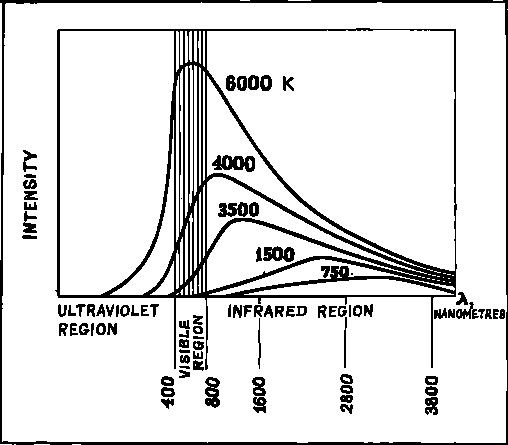
\includegraphics[width=0.9\textwidth]{figures/fig-01-01.pdf}
\caption{Theoretical spectrum of an incandescent (black) body for several temperatures.}
\label{fig-1.1}
\end{figure}


It is well to point out here that the derivation of the shape of this curve (this was done by Max Planck in 1900) was the first step in the development of quantum physics. In order to obtain agreement of theory with experiment, Planck had to assume that radiation and absorption of light take place in separate portions. Planck was not prepared to take the next step and state that we are justified in speaking of particles of light (photons). That step was taken by Albert Einstein in 1905.

It was only in 1913 that Niels Bohr introduced the concept of quantization of energy. And if we want a logically rigorous theory of thermal radiation, the year of birth can be put as 1926.

Let's first discuss the shapes of the curves and only then talk about theory. First of all, note that as the temperature rises, the area under the curve rapidly increases. What is the physical meaning of the area bounded by the radiation curve? When constructing curves similar to those depicted in the figure, we say that the intensity of radiation for a given wavelength is laid off on the axis of ordinates (horizontal axis). But what does a ``given wavelength'' mean? Do we mean 453 or 453.2 nanometres? Maybe \num{453.257859987654}? It is probably clear that when we speak of a ``given wavelength'', we mean a very small interval of wavelengths. We agree, say, that the interval is equal to 0.01 nanometre. From this it follows that it is not the ordinate that has physical meaning but a tiny column with a base of 0.01 nanometre. The area of this column is equal to the energy radiated by the waves having lengths in that interval (for example, from 453.25 to 453.26 nanometres). Now if we break up the whole area into such columns, we get the total intensity of the whole spectrum. That is precisely the operation mathematicians perform and it is called integration. To summarize: the area under our curve yields the total intensity of the radiation, and it turns out to be proportional to the fourth power of the temperature.


In the figure we are discussing it is clear that with increasing temperature there is not only a change in the area occupied by the curve but there is a shift of its maximum to the left, that is, into the region of ultraviolet radiation.

The relationship between the wavelength of light in micrometres that corresponds to the greatest intensity of radiation (or absorption) and the temperature in kelvins is given by the following formula:
\begin{equation*}%
\lambda_{\textrm{max}} = \frac{2886}{T}
\label{lambdamax}
\end{equation*}
At the lowest temperatures, the maximum lies in the infrared region. That is precisely why infrared radiation is also termed thermal radiation. And it is a marvelous thing that we have instruments capable of sensing the thermal radiation emitted by bodies at room temperature and even lower. There are instruments today that can see in total darkness. Some animals, by the way, have the same capability. There is nothing at all strange in this fact since infrared rays have, in principle, the same properties as visible rays.

Also, don't forget that every animal is a source of radiation. We sometimes hear of a person being able to ``feel'' the presence of another person in darkness. No mysticism is involved, merely the one who ``feels'' has a highly sensitive perception of thermal rays.


%\newpage
\begin{center}
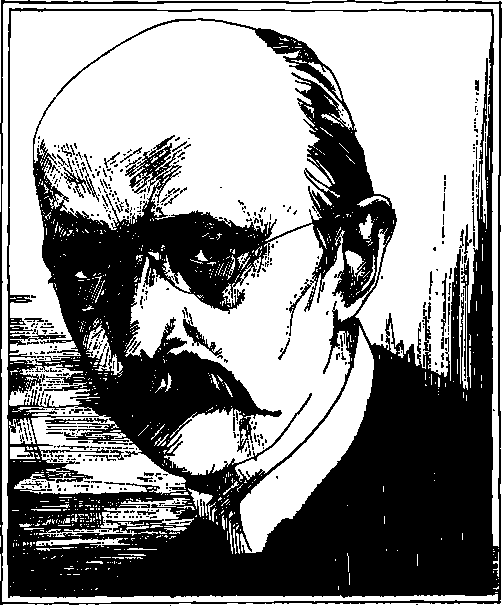
\includegraphics[width=0.8\textwidth]{figures/planck.pdf}
\end{center}
{\small \textsf{{Max Planck [1858-1947]}} -- \textsf{\footnotesize outstanding German scientist who laid the foundations of quantum theory. In an attempt to find a mathematical expression for a proper description of the spectral distribution of the emission of an ideal black body Planck demonstrated that such a formula could be obtained by introducing a ``quantum of action''. Planck assumed that a body emits energy in parcels, equal to the product of a constant (which later was named after him) by the frequency of the light.}}



I can't resist telling the reader about an interesting episode that demonstrates the necessity of taking thermal rays into account even when, in the very ordinary sense of this word, the source of rays is not a heated body. A few years ago I was asked to investigate some experiments conducted by a person who considered himself a magician capable of stopping a motor using only his will power.

My task was to find a rational explanation (sorcerers of the twentieth like to deal in pseudoscientific terminology and so call these experiments telekinesis).

\begin{figure}[!ht]
\centering
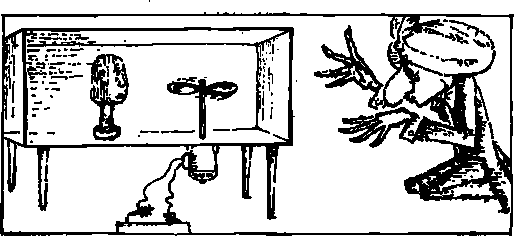
\includegraphics[width=\textwidth]{figures/fig-01-02.pdf}
\caption{Deciphering the sorcerer's trick.}
\label{fig-1.2}
\end{figure}

A diagram of the experiment is shown in \figr{fig-1.2}. A wing was set in rotation by a small motor, and the wing really did stop whenever the magician sat down next to the box where the axle of the motor emerged from below. I soon found that anybody who sat down in that position would be able to stop the wing. It usually took about 10 to 15 minutes to perform the operation. And it wasn’t the motor that came to a halt, as the magician claimed, but the little wing. It was clear then that some kind of force connected with the human body was interfering with the force of adhesion between the axle of the motor and the wing.

I pointed out that the wing could be stopped almost instantly if an electric lamp were brought up close to the side of the box. It was obvious that the trick lay in the heat emitted by the human body. I sent a whiff of tobacco smoke into the box and demonstrated that the convection currents of air inside the box move so as to prevent the wing from rotating. Exact measurements showed that the temperature of the side of the box closest to the human body is about one degree higher than the opposite side. Infrared rays emitted by a body heated to 60-70 degrees Celsius can be felt if the hand is held at a short distance. Thermal convection of course must be eliminated. Heated air rises upwards, so bring your hand close from below. You will then be certain that you are perceiving thermal rays.

We conclude our talk about thermal rays with an explanation of why the modern electric light bulb with a tungsten filament is a great step beyond a bulb with a carbon filament. The whole point is that a carbon filament can be heated to \SI{2100}{\kelvin}, while a tungsten filament can be heated all the way up to \SI{2500}{\kelvin}. Why are these 400 degrees so important? Because the purpose of an incandescent lamp is to provide light and not heat, and so the aim is to have the maximum of the curve located in the visible portion of the radiation. It will
be seen from the graph that the ideal is to have a filament that can withstand the temperature of the Sun's surface, or \SI{6000}{\kelvin}. But even the step from 2100 degrees to 2500 degrees raises the portion of energy involving visible radiation from 0.5\% to 1.6\%.

\section{The Theory of Thermal Radiation}
If a system of radiating and absorbing bodies is closed, then the photon ``gas'' (with the aid of which the bodies exchange energy) must be in equilibrium with the atoms supplying the photons. The number of photons with energy $h\nu$ depends on how many atoms lie in the $E_{1}$ level and how many in the $E_{2}$ level. In the case of equilibrium, these numbers remain unchanged.

However, the equilibrium is of a dynamic nature since the processes of excitation and radiation occur at the same time. In some way (either by collision with another particle or due to absorption of a photon from without) the atom or the atomic system climbs to a high level. The system persists in this excited state for some (in definite) time (ordinarily for a fraction of a second) and then reverts to a low level. This process is termed \emph{spontaneous radiation}. The atom behaves like a little ball on the top of a sharp peak with an intricate configuration: the slightest breath of air is enough to disrupt the equilibrium. The ball rolls down into a valley, usually the lowest part, and then only a strong impact can bring it out again. We say that an atom that has dropped to the lowest level is in a stable state.

But here we must bear in mind that there are also intermediate states in between the peak and the lowest portion of the valley. The ball may be at rest in a slight depression from which it can be extricated by a waft of air, so to speak, or at least by a little push. This is a metastable state. Thus, besides the excited and stable states there is a third, metastable, type of energy level.

To summarize, then, the transitions will occur in both directions. First one atom and then another atom will move into a higher level. In the next instant, they will fall to a lower level and emit light. But at the very same time, other atoms will receive energy and will rise to upper levels.

The law of conservation of energy requires that the number of transitions upwards equal the number of transitions downwards. What does the number of transitions upwards depend on? Two factors: first, the number of atoms in the lowest floor, and, second, the number of impacts that raise them to a higher floor. And the number downwards? It is of course determined by the number of atoms lying in the upper floor, and it would seem to be in dependent of any other factors. That is precisely what theoretical physicists thought at first, and yet the pieces didn’t fit. The number of transitions upwards, which is dependent on two factors, increased with temperature much faster than the number of transitions downwards, which is dependent on only one factor. This model, which had appeared to be so obvious, turned out to be nonsense: Sooner or later all the atoms would be chased up to the highest level: the system of atoms would be in an unstable state with no radiation.

It was precisely this impossible conclusion that Einstein, in 1926, picked up from the reasoning of his predecessors. Apparently, there was some other influence affecting the transitions of atoms from the upper floor to the lower floor. One could only conclude that there is a forced transition in addition to the spontaneous transition to the lower level.

What is this \emph{stimulated emission}, as it is called? In short, it is this. A system is in the upper level. It is separated from the lower level by the difference $E_{2} - E_{1}= h\nu$. Now, if a photon with energy $h\nu$ is incident on the system, then it makes the system move down to a lower level. The incident photon is not absorbed in the process but continues onwards accompanied by a fresh photon of exactly the same kind generated by the first one.

Do not seek any logic in this reasoning. It was intuition, a guess and experiment was to prove it right or wrong. Using the assumption of stimulated emission we are able to derive a quantitative formula that yields the graph of emission as a function of the wavelength of a heated body. The theory proved to be in brilliant agreement with experiment and so justified the hypothesis.

It is an exciting thought that the practical conclusions from the fact of the existence of stimulated emission that led to the invention of lasers were drawn only many years later.

\section{Optical Spectra}

Generally speaking, any body is a source of soft electromagnetic radiation. Using a spectrograph (this is an instrument whose principal component is a prism or a diffraction grating), light can be decomposed into a spectrum. The spectrum may turn out to be continuous, banded or line. The spectra of incandescent solids are very similar. For that matter, only a few substances can be heated to incandescence. A real rarity is a glowing liquid. The emission spectra of gases are highly informative. Such are the spectra of rays coming to us from distant stars. The bulk of the information we have concerning the structure of the universe comes to earth in the form of light rays of stellar matter in a gaseous state.

Under terrestrial conditions, it is easy to obtain emission spectra of atoms. Atoms are made to glow either by passing a current through the gas or by heating. In this manner we can obtain only the spectra of atoms but not the spectra of molecules. Before the gas begins to glow, the molecules break up into atoms. That is why absorption spectra are studied if the investigator is interested in liquids or solids. In the final analysis, the picture is determined by the system of energy levels. Transitions up or down yield the same information. Simply, do what is easiest.

Spectra that consist of separate clear-cut lines can be obtained only from a gas or a diluted solution. In the second book of this series it was stated that the behaviour of dissolved molecules resembles in many respects the behaviour of a gas. This also holds true for optical spectroscopy. Unfortunately, the solvent affects the character of the spectrum, but if we compare the type of spectra of molecules dissolved in different substances, it is possible to take that effect into account and extract from the experiment the fingerprints of the dissolved molecule.
%\newpage
\begin{center}
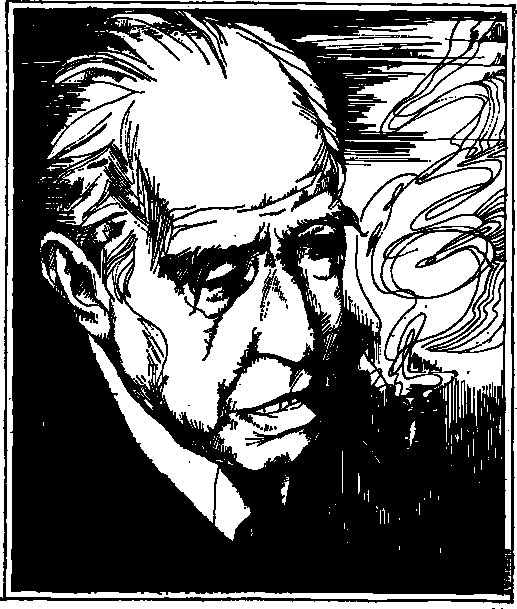
\includegraphics[width=0.8\textwidth]{figures/bohr.pdf}
\end{center}
{\small \textsf{{Niels Bohr [1885-1962]}} -- \textsf{\footnotesize the famous Danish physicist who creat­ed the first quantum model of the atom and thus discovered the law of quantization of energy. He was an active participant in developing the principles of quantum mechanics. He demonstrated the fundamental inapplicability -- to the microworld -- of concepts suitable in describing the behaviour of macroscopic bodies. He made a very considerable contribution to the theory of the structure of the atomic nucleus.}}

Obtaining a characteristic spectrum does not mean establishing the system of energy levels of a molecule. But for many practical purposes this is not required. With an album of information about spectra (that is, the list of spectral lines and their intensities, or the curves of intensity versus frequency) of some family of chemical substances, we can, by taking the spectrum of an unknown substance and comparing the experimental pattern with material from the album, determine the substance in the very same way that a criminal is detected from the fingerprints he leaves.


Just lately, optical spectral analysis has come up against a competitor: radiospectroscopy. Radio spectroscopic methods are still inferior in sensitivity to optical methods (though the inferiority will most likely not last long) but are far superior to optical methods in the identification and quantitative analysis of mixtures of substances.


We don’t aim here to acquaint the reader with concrete spectra of substances. It will suffice to discuss the pattern of energy levels of atoms of hydrogen and the fundamental scheme of energy levels of a free molecule.
\begin{figure}[!ht]
\centering
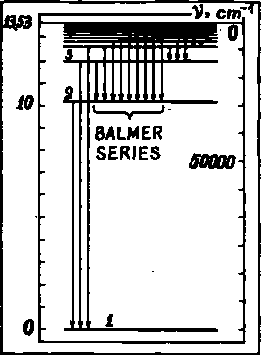
\includegraphics[width=0.5\textwidth]{figures/fig-01-03.pdf}
\caption{System of energy levels of hydrogen.}
\label{fig-1.3}
\end{figure}

\figr{fig-1.3} depicts the system of energy levels of hydrogen. Note the characteristic thickening of levels as we move away from the zero line.

Incidentally, the zero in the diagram is not a ``real'' zero actually. An unexcited atom of hydrogen naturally possesses some energy. But since spectra exhibit energy differences, it is convenient to reckon energies from the lower line. Depending on the intensity of the ``shock'' obtained, the atom can rise to any one of the ``floors'', hold on for a moment in the nonequilibrium state and then, via one of two possible modes (spontaneous emission or stimulated emission), revert to the lower level.

The resulting spectrum may conveniently be split up into a number of series. Each series is subordinate to its lower level. In the visible portion of the spectrum we have the so-called \emph{Balmer series}. The explanation of this series was the first triumph of Niels Bohr's theory of atomic structure.


Not all energy transitions are of equal probability. The higher the probability of transition, the more intense the appropriate line. There are also forbidden transitions.

A great achievement of theoretical physics was the exhaustive interpretation of the spectrum of the hydrogen atom via the solution of the famous equation of quantum mechanics derived in 1926 by the Austrian physicist Erwin Schr\"odinger (1887-1961).

Atomic spectra are affected by external fields. The lines split into several components under the action of an electric field (the \emph{Stark effect}) and under the action of a magnetic field (the \emph{Zeeman effect}). We will not go into these exciting phenomena here, but it is necessary to point out that an understanding of them came only after Samuel Goudsmit and George Uhlenbeck made the assumption that the electron possesses spin. How spin reveals itself in experiment directly was discussed in the third book of this series.

And finally the last remark regarding the pattern of energy levels. We see that the limit which the levels come up to is marked by the number 13.53. What kind of number is this? This is the \emph{ionization potential}. If we multiply the electron charge by the magnitude of this potential in volts, we obtain the amount of work needed to tear the electron away from the nucleus; in other words, this is the work that must be done to destroy the hydrogen atom.


Atomic spectra arise as a result of electron transitions. As soon as we move from atoms to a molecule, we immediately have to take into account two more components of energy. A molecule can rotate and the atoms of a molecule can perform vibrations with respect to one another. All these types of energy can likewise be quantized, which means they can have only specific discrete values. Thus, the energy state of a molecule is described by the state of its electron cloud (\emph{electronic level}), the state of oscillatory motion (\emph{vibrational level}), and the state of rotation (\emph{rotational level}). We thus have to deal with three kinds of information: the number of the house, the floor, and the flat.

\begin{figure}[!ht]
\centering
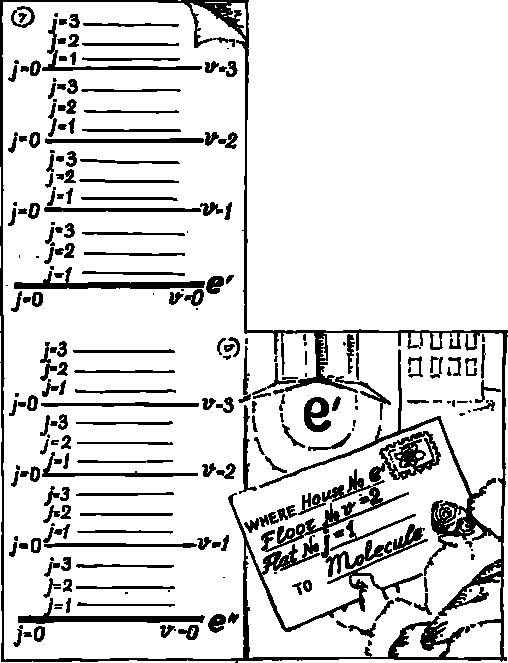
\includegraphics[width=0.8\textwidth]{figures/fig-01-04.pdf}
\caption{Schematic of electronic transfers in an atom with the required information.}
\label{fig-1.4}
\end{figure}

But what is the role of the ``floor'' and the ``flat''? What energy levels have big separations and what levels have small separations? All these questions are answered in \figr{fig-1.4}. This diagram shows two electronic levels $e'$ and $e''$ (the house numbers). The floors are the vibrational levels marked $\nu$, and the numbers of the flats are the rotational levels marked $j$. True, this differs somewhat from the ordinary numbering of houses and flats, which is continuous; in dealing with molecular spectra we number the flats on every floor from zero. Thus we see that the gaps between rotational levels are the smallest and between electronic levels ($e'$ and $e''$) the largest.

Suppose a molecule has the following possible electronic levels: 100, 200, 300, units of energy, vibrational levels at 10, 20, 30, \ldots\, units of energy, and rotational levels at 1, 2, 3, \ldots\, units of energy; then a molecule on the second electronic level, the first vibrational level, and the third rotational level will have an energy of 213 units.

Thus, we can give the energy of a molecule as follows:
\begin{equation*}%
W = W_{\textrm{el}} + W_{\textrm{vib}} + W_{\textrm{rot}}
\end{equation*}
The frequency of the emitted or absorbed light will always correspond to the difference (symbol: $\Delta$) of two levels:
\begin{equation*}%
\nu = \frac{1}{h} \left( \Delta W_{\textrm{el}} + \Delta W_{\textrm{vib}} + \Delta W_{\textrm{rot}} \right)
\end{equation*}

I would like to touch on those transitions that involve a change in only one type of energy. In practice, this occurs only in the case of rotational transitions, and why this is so will soon be seen.

We begin our investigation with the absorption of electromagnetic waves of a group of molecules starting with the longest wavelengths, that is, with the smallest portions of energy $h\nu$. Until the magnitude of the energy quantum has become equal to the distance between the two closest-lying levels, the molecule will not begin to absorb. By gradually increasing the frequency, we will reach quanta capable of raising the molecule from one ``rotational'' step to the next. Experiment shows that this occurs in the region of microwaves (the edge of the radio spectrum) or, to put it differently, in the region of the far infrared spectrum. Wavelengths of the order of 0.1 to 1 millimetre will be absorbed by the molecules. What we then have is a purely band spectrum.

New things happen when we irradiate the substance with energy quanta sufficiently high to move the molecule from one vibrational level to another. However, we will never attain a purely vibrational spectrum, that is, a series of transitions under which the number of the rotational level is preserved. On the contrary, transitions from one vibrational level to another will involve a variety of rotational levels. Say, a transition from the zero (lowest) vibrational level to the first can consist in moving up from the third rotational level to the second, or from the second to the first, and so forth. We thus obtain a vibration-rotation spectrum. We observe it in infrared light (from 3 to 50 micrometres). All transitions from one vibrational level to another will differ slightly in energy and will yield a group of very close lines in the spectrum. In the case of small resolution, these lines merge into a single band. Each band corresponds to a definite vibrational transition.

We thus move into a new spectral region, the region of visible light where the energy of the quantum becomes sufficient to move the molecule from one electronic level to another. Of course, it is not possible here to obtain either purely electron transitions or electron-vibrational transitions. Complex transitions arise in which the energy transition is accompanied by a change in the ``house'', the ``floor'',and the ``flat''. Since a vibrational-rotational transition constitutes a band, the spectrum in the visible region will be practically continuous.

The characteristic spectra of atoms and molecules have for many years played the role of helpers in determining the chemical structure and composition of substances. And their aid continues today. Revolutionary events in the field of spectroscopy have only just recently occurred.

\section{Laser Radiation}

The first thirty years of this century saw fantastic advances in theoretical physics with the discovery of such important laws of nature as the laws of the mechanics of high velocities, the laws of the structure of the atomic nucleus, and the laws of quantum mechanics. And the forty years that followed exhibited just as phenomenal a development in the applications of theory to practice.

This was a time when humanity harnessed the energy of atomic nuclei and invented semiconductor transistors that revolutionized radio engineering and led to the development of electronic computers and laser technology. These three applications were actually what produced the modern revolution in science and engineering.

In this section we discuss lasers. First let us give some thought to the problem of why, operating via traditional methods, we are not able to generate an intense directed beam of light.

The strongest stream of light collected into a very narrow beam disperses and loses its energy over small distances. It was only in the science fiction of the Russian writer Aleksei Tolstoi that the hero devises a ``hyperboloid'' capable of generating bursts of intense light rays that can burn and cut materials and carry tremendous energy over great distances. Of course we know that it is possible to manufacture a concave mirror that can generate a parallel beam of light. This requires placing a point source in the focus of the mirror. But a point is a mathematical abstraction. All right, suppose we have a small source, bigger than a point. But even then, if we heat the ball to 6000 degrees (and no known material can stand more), we obtain a beam of light of miserably low intensity. And as soon as we increase the dimensions of the source, then instead of a parallel beam of rays we obtain a spread-out fan of light ``filaments'' and the intensity of the ray of the projector begins to rapidly diminish with distance.

Thus, the first obstacle to creating a strong beam of light is that atoms emit light in all directions. That’s the first, but not the last. Atoms and molecules emit light without agreeing on how they’ll do it. The result is that rays from different atoms set out at different times, totally unmatched in their efforts. The emissions of different atoms do not agree in phase, and that means that rays from different atoms will frequently annihilate one another. This occurs, as you will recall, when the hump of one wave comes with the valley of another one.

\emph{Laser emission} is what overcomes these obstacles. The word ``laser'' stands for \textbf{l}ight \textbf{a}mplification by \textbf{s}timulated \textbf{e}mission of \textbf{r}adiation.

The underlying idea is made up of several elements. First of all, recall that there is stimulated emission and spontaneous radiation. We have already mentioned that this type of emission occurs when a light photon encounters an excited atom. If the excitation energy of the atom is exactly equal to the energy of the photon, then the photon de-excites the atom, which moves to a lower level and emits a photon. The marvelous peculiarity of stimulated emission is that the new photon is the same as the one that generated it, and not only in energy but also in phase and direction of motion.

The second element behind this idea is this. If the system of emitting atoms is placed in a tube, the ends of which are at a certain distance from each other and can serve as mirrors for the photons that interest us, then we can build up a bunch of photons generated (as they move back and forth) by identically excited atoms.
The third element in this idea is to retain the atoms in the excited state as long as possible and then, after the pumping is completed, to force all atoms to de-excite at the same time. Putting this laser idea (that is, the production of millions upon millions of identical photons from a single photon) into hardware should permit generating a light beam of unimaginable intensity. Such a beam would exhibit only the slightest spread and would have tremendous energy over its cross section.

But the question is: How can this be attained? For decades no one knew. Back in the 1930s, important ideas in this connection were expressed by Soviet physicist V. A. Fabrikant. Later, persistent research of Soviet scientists A. M. Prokhorov and N. G. Basov and, independently, the American physicist Charles Hard Townes led to the invention of lasers. All three received the Nobel prize in physics.

\begin{figure}[!ht]
\centering
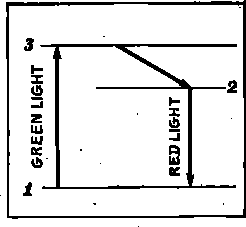
\includegraphics[width=0.4\textwidth]{figures/fig-01-05.pdf}
\caption{Two level system for laser processes.}
\label{fig-1.5}
\end{figure}

Suppose a system has two energy levels. Most atoms or molecules are in the lower level. Thermal shocks can transfer a molecule to the upper level for a short time. But not for long, because the molecule is de-excited. In the process most of atoms go to the lower level spontaneously. Of course, some of emitted photons will carry some of the excited atoms to the lower state and generate photons of stimulated emission. But these are rare processes because there are few excited particles (the most occupied are the lower levels), and also the probability of a spontaneous transition is substantially higher than the probability of stimulated emission.

Let us suppose it was possible to find a substance whose atoms have the three energy levels marked in \figr{fig-1.5} by the numerals 1, 2, and 3. The distance 1-3 corresponds to the frequency of emission of green light, the distance 1-2 corresponds to the frequency of red light. Now suppose the probability of a transition from level 3 to level 2 is thousands of times higher than the frequency of transitions from level 2 to level 1. Let us irradiate the substance with green light. The atoms will rise to the third floor, then via spontaneous transitions will go to level 2 and will stay at that level. This is termed \emph{nonradiative transition}. The energy released goes into the vibrational energy of the atoms. Using our imagination further, let us suppose that we have carried most of the atoms to level 2. We have thus reversed the occupancy density, it is no longer ``normal''. There are more in the upper levels 2 than in the lower levels 1, which is impossible when the process is controlled solely by thermal motion.

And still and all there does begin a transition from level 2 to the lower level 1. An appropriate photon will encounter other atoms in the excited level 2. The result will be not absorption but the creation of a new photon. The first, accidentally generated photon in 2-1 will be joined by the very same photons of stimulated emission.

Thus arises a stream of 2-1 photons. They will all be identical and will generate a beam of tremendous intensity.

That precisely was the process that the three Nobel prize winners were able to create. Historically, the first was a ruby laser. The diagram of levels shown in the figure is precisely the diagram of ruby with an admixture of chromium atoms.

To make a laser we need a source of excitation that does the pumping of the laser, that is, that carries the atoms to higher levels.

If the source of laser emission is a solid, then it is made in the form of a cylinder whose bases play the part of mirrors. In the case of a liquid or gaseous laser, a tube is constructed with mirrors at the ends of the column. By performing a micrometre-precise positioning of the mirrors and thus fixing the length of the column, we put in a privileged position only those photons whose integer number of wavelengths fit into the length of the column. Only then do all the waves combine.

Perhaps the main peculiarity of the laser is the possibility of creating a narrow stream of radiation. Practically speaking, a laser beam can have almost any cross section. Technically, this is achieved by the fact that the ray is made to travel along a narrow glass capillary tube of sufficient length. Photons moving at an angle to the capillary do not participate in the photon build-up. A resonance cavity (that is, the mirrors that reflect photons first in one direction and then in the other during the pumping period in the operation of the laser) reproduces photons of only one direction. In some cases, if an angular dispersion of the beam of the order of one degree is not satisfactory, a supplementary lens is placed in the path of the released ray.

A laser device is a complicated piece of engineering if one has to do with high power outputs. A primary pulse is first set up in the column; then it is fed to amplifiers that function in the same manner as the first column but pump independently of the first column. We will not go into these details because we are only interested in the physical principles of pumping and the generation of laser emission. They can differ greatly, as is evident from a glance at \figr{fig-1.6} to \figr{fig-1.8} with diagrams of the action of lasers which today yield beams of maximum power output.

\begin{figure}[!ht]
\centering
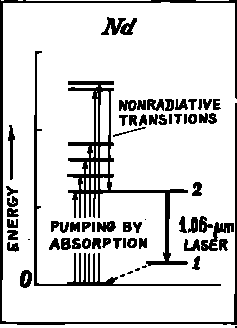
\includegraphics[width=0.4\textwidth]{figures/fig-01-06.pdf}
\caption{Schematic of a neodymium laser.}
\label{fig-1.6}
\end{figure}


\figr{fig-1.6} depicts a so-called neodymium laser. Actually, the body of the laser is not the metal neodymium but ordinary glass with an admixture of neodymium. Ions of neodymium atoms are haphazardly distributed among the atoms of silicon and oxygen. Pumping is performed by flash bulbs. The lamps emit in wavelengths between 0.5 and 0.9 micrometre, and a broad band of excited states is obtained (shown here in the form of five bars). The atoms perform nonradiative transitions to the upper laser level (labelled 2 in all three figures). Each transition yields a different energy, which is converted into the vibrational energy of the whole ``lattice'' of atoms.

Laser emission, that is, the transition to an empty lower level labelled 1, has a wavelength of 1.06 micro metres. 

The dashed line, which depicts the transition from level 1 to the lowest level ``does not work'' (in the sense that energy is released in the form of noncoherent radiation).

A neodymium laser permits obtaining fantastic power outputs of up to \SI{d12}{\watt}. The energy is generated in the form of pulses lasting 0.1 nanosecond.

\begin{figure}[!ht]
\centering
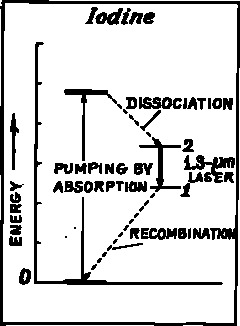
\includegraphics[width=0.4\textwidth]{figures/fig-01-07.pdf}
\caption{Schematic of an iodine laser.}
\label{fig-1.7}
\end{figure}

A new competitor in this field is a laser using transitions in excited atoms of iodine (\figr{fig-1.7}). The working substance here is the gas \ce{C3F7I}. Here, too, flash bulbs are used for pumping, but the physical processes are different. Ultraviolet light of wavelength 0.25 micrometre is used for pumping. Under the action of this radiation there occurs a dissociation of the molecules. The remarkable thing is that the iodine atoms are torn out of the molecule and are in an excited state! As the reader will see, this is quite a different method for inverting the occupancy density. The operating transition $2 \to 1$ leads to laser emission with a wavelength of 1.3 micrometres, after which the iodine atom joins up with the molecular residue.

The reader has also probably heard of the widespread use of helium-neon lasers. They are used to obtain an intense infrared ray of wavelength 1.13 micrometres. These lasers are not record holders as far as power goes, and so we give a diagram of levels for a different laser that operates on a mixture of nitrogen and carbon dioxide (\figr{fig-1.8}).

\begin{figure}[!ht]
\centering
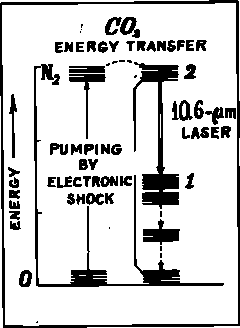
\includegraphics[width=0.4\textwidth]{figures/fig-01-08.pdf}
\caption{Schematic of nitrogen and carbon dioxide based laser.}
\label{fig-1.8}
\end{figure}
Before describing this laser, a natural question comes to mind, and that is: Why are mixtures of gases needed? The point is that some atoms and molecules are more easily excited while others are more easily de-excited, so that in a laser operating on a mixture, particles of one type effect the pumping process, these then transfer the energy via collisions to other atoms or molecules, and these in turn generate the laser beam. There are systems now functioning that consist of more than two gases.
For instance, in the nitrogen-carbon dioxide laser, it is advisable to add a variety of components including helium.

Pumping in the \ce{CO2} laser is done differently from the two just described. The mixture of gases is placed in a gas-discharge tube and a sufficiently high voltage is applied so that the system becomes a plasma. Electrons moving at high speeds excite the vibrations of nitrogen molecules. The diagram shows a transition of this molecule to the upper floor. The voltage applied to the electrodes plays a delicate role. The optimal energy for exciting nitrogen molecules is about \SI{2}{\electronvolt}. The nitrogen molecule is only an intermediary. It does not by itself produce any emission but rather transfers the energy obtained from the electrons to the \ce{CO2} molecule and lifts it to an upper laser level.

The upper laser levels 2 are ``flats of the third floor'' of \ce{CO2} molecules. A molecule of gas has a lifetime in the upper laser level equal to about 0.001 second. This is not so little, and the molecule has a good chance of encountering a photon of suitable energy that will force it down to a lower level.

It should be pointed out that ``interflat'' transitions are a much more frequent occurrence than ``interfloor'' transitions. Lifetimes on the rotational level are of the order of ten millionths of a second. This favourable circumstance results in the flats of each floor being occupied in a rather stable fashion, and so, using an engineering technique that we have already mentioned (setting a suitable distance between the mirrors), it is possible to isolate some one transition; let us say, from the sixth flat of the third floor to the fifth flat of the second floor.

The designing engineer must have at his disposal complete information about the residence time of an atom on any given sublevel and about the probabilities of transition. Then he is able to choose the optimal radiation of the given gaseous mixture. Ordinarily, a laser operating on carbon dioxide is tuned to a wavelength of \num{10.5915} micrometres. For a laser to function normally, it is necessary that the molecules not pile up on the lowest laser level, the idea being for them to do their jobs and get out. Now, at a gas pressure of 1 millimetre of mercury, carbon dioxide molecules experience 100 collisions per second in vacating the level. The respective figures are \num{4000} and \num{100000} if helium and water are present. This is a tremendous difference.

By selecting the proper admixtures for carbon dioxide, we can boost the power output of the instrument substantially. It would appear that this is the gold-medal winner in the laser field.

A carbon dioxide (\ce{CO2}) laser produces a beam that can be focussed on an area of \SI{0.001}{\centi\meter\squared} with an intensity of \SI{1000}{\kilo\watt\per\centi\meter\squared} in continuous operation and one million \si{\kilo\watt\per\centi\meter\squared} in pulsed operation with the pulse time equal to one nanosecond (which, as you know, is \num{d-9}, or one thousand millionth, of a second).

The search for suitable materials for lasers is a sort of art. One needs intuition, ingenuity, and memory to create an effectively operating laser. The user can now order lasers with a great variety of wavelengths ranging from a tenth of a micrometre to hundreds of micrometres.

The exceptional intensity and coherence of laser emission have revolutionized many areas of engineering. During the past decade, the manufacture of lasers has become a whole industry. Lasers have found application as generators of radiation that trasmit not only energy but also information. Intense research is in progress for their use in initiating thermonuclear reactions. Lasers are used in place of the surgeon's knife in medicine, as an instrument for the most delicate surgical operations, as a device for the separation of isotopes. We will have occasion later on to come back to further discussions of the marvelous laser.

\section{Luminiscence}
Thermal radiation is a universal property of all bodies. Thermal rays are emitted by every body at any temperature from absolute zero upwards. The thermal spectrum is a continuous one and is depicted by a curve that we have already discussed. True, our curve was that of a black body, but the behaviour of coloured bodies is in principle but slightly different from the behaviour of black bodies. Merely, the curve for coloured bodies is distorted somewhat. But the general increase in the energy of emission (as the temperature rises) and the displacement of the maximum to the left (if wavelengths are laid off on the axis of abscissas) are the general law.

All radiation consists in a transition from a higher energy level to a lower level. But the reasons for excitation of atoms or molecules may differ. In the case of
thermal radiation, it is the collisions of particles of the substance due to thermal motion.

But that is not the only reason compelling a body to emit waves. \emph{Luminescence}, which we are about to discuss, is of a different nature. This term embraces processes of excitation of molecules that are not connected with any increase in the temperature of the body. Causes of particle excitation may be encounters with beams of photons or electrons, mechanical impact, friction, and so on.

Practically all substances are capable of luminescence. But only some (called luminophors or phosphors) glow brightly and are of practical importance.

Luminophors are used as materials for covering television and oscillograph screens, in which case the luminescence occurs under the impact of electrons. Certain substances luminesce brightly under the action of ultraviolet radiation. The energy of the incident photon must be at least greater than the energy of the emitted photon. That is why the incident quantum of energy can come from the invisible portion of the spectrum while the emitted radiation can lie in the visible portion.

Admixtures of luminescent material measured in minute fractions (billionths, or \num{d-9}) are sufficient to make a substance luminesce under irradiation by ultraviolet light. That is why fluorometric analysis is sometimes used as a tool in chemical analysis. It is capable of detecting minute quantities of impurities.

Luminophors are used to cover the walls of daylight lamps.

There are two types of luminescence: fluorescence and phosphorescence. \emph{Fluorescence} consists in the de-excitation of an atom or molecule that occurs without the molecule remaining in the excited level. Contrariwise, \emph{phosphorescence} persists after the excitation has ceased. This occurs if the system, when excited, passes to a metastable level, from which transitions downwards have a low probability. As a rule, the radiation occurs after the molecule first absorbs the energy and rises to a higher level, after which de-excitation takes place, the transition to the lower level occurring without any stop at an intermediate, metastable, level.

A few words about \emph{electroluminescence} that occurs in certain semiconductor diodes on the boundary of a $p\!-	\!n$ region. This interesting phenomenon is of great practical value because it underlies the manufacture of semiconductor lasers. The idea is this: an electron and hole of the semiconductor can recombine with the emission of a photon.

For transitions of this type to take place continuously we have to pass an electric current through the diode. The problem is to find a suitable material that satisfies several requirements. First of all, the current has to inject (if that is the word) electrons into the $p$-type semiconductor material, that is, a semiconductor containing more holes, or it must pump holes into an $n$-type crystal. This is a necessary condition, but other factors such as, for example, the rate of transition from an upper to a lower level can play a decisive role. Then there are cases where all factors favour a transition of an electron downwards and electroluminescence takes place.

A particularly good electroluminescent material is the semiconductor gallium arsenide. It yields a sufficient quantity of photons. The photons move along the $p\!-\!n$ boundary. Two sections of the diode perpendicular to the boundary are polished and that sets up a resonant cavity. The photons generated in recombinations of holes and electrons are in phase, and for sufficiently large currents the radiation becomes stimulated emission with all the resultant consequences of being narrow, highly directed, and polarized.

Semiconductor lasers operate in a band of wavelengths from the ultraviolet to the far infrared and are widely used for a variety of purposes.


%\begin{figure}[!ht]
%\centering
%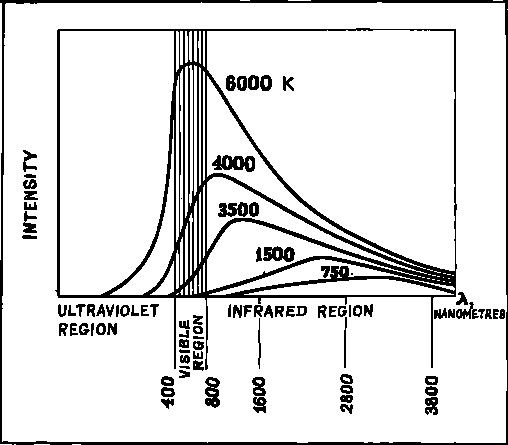
\includegraphics[width=\textwidth]{figures/fig-01-01.pdf}
%\caption{Using springs for measuring weights.}
%\label{fig-1.1}
%\end{figure}



